\documentclass{article}

%<<setup, include=FALSE>>=
%library(knitr)
%@
\title{Simple Regression Analysis}

\author{Thomas Sun}

\date{October 31, 2016}

\usepackage{Sweave}
\begin{document}
\Sconcordance{concordance:lab9.tex:lab9.Rnw:%
1 11 1 1 0 32 1 1 7 12 0 1 2 4 1 1 10 14 0 1 2 13 1}

\maketitle


\begin{abstract}

This report attempts to reproduce the results found in Chapter 3 of the book \textbf{An Introduction to Statistical Learning}. In this chapter, a regression analysis is run on the \textit{Advertising} dataset, containing data on sales and advertising budget for a particular product. Using a simple linear regression model, I find the same estimates of the coefficients, obtain the same quality index results, and similar looking plots as the ones contained in the book.

\end{abstract}

\section{Introduction}

The goal is to determine whether there is an effect of advertising on sales, ideally to increase product sales. Specifically, if increasing spending on certain mediums of advertising has a relationship with the amount of sales on a product. The chapter mainly considers one medium, \texttt{TV}, and fits a regression model to it with \texttt{Sales}. It finds that there is a strong positive relationship between \texttt{TV} and \texttt{Sales} and the data points fit the regression line closely.

\section{Data}

Data was obtained by downloading the \textit{Advertising} dataset available on the textbook's website. It contains data of the size of advertising budget for \texttt{TV}, \texttt{Radio}, and \texttt{Newspaper} (in thousands of dollars) for a product in 200 different markets, in addition to the number of sales (in thousands of units) for the product in each market. We specifically are interested in the data for \texttt{TV} and \texttt{Sales}.

\section{Methodology}

In order to estimate the relationship between \texttt{TV} and \texttt{Sales}, a simple linear model is used.

\begin{equation}
Sales = \beta_0 + \beta_1 TV
\end{equation}

Where $\beta_0$ and $\beta_1$ are the regression coefficients, intercept and slope, respectively. To find an estimate for these coefficients, we use the ordinary least squares method to fit the model. OLS regression was run through RStudio, where the regression coefficients and quality indices (mean squared error, R-squared, F-statistic) are calculated. We also plot \texttt{TV} against \texttt{Sales} to replicate the scatterplot in the chapter.

\section{Results}

The estimated coefficients were calculated and found on the following table.

% latex table generated in R 3.1.1 by xtable 1.8-2 package
% Mon Oct 31 11:03:19 2016
\begin{table}[ht]
\centering
\begin{tabular}{rrrrr}
  \hline
 & Estimate & Std. Error & t value & Pr($>$$|$t$|$) \\ 
  \hline
(Intercept) & 7.033 & 0.458 & 15.360 & 0.000 \\ 
  TV & 0.048 & 0.003 & 17.668 & 0.000 \\ 
   \hline
\end{tabular}
\caption{Regression Coefficients} 
\end{table}


Both estimators have low standard deviation and p-value of practially zero, suggesting these calculated values are very statistically significant. In order to assess the fit of the data with the regression line, the following measurements were calculated in the table below.

% latex table generated in R 3.1.1 by xtable 1.8-2 package
% Mon Oct 31 11:03:19 2016
\begin{table}[ht]
\centering
\begin{tabular}{rr}
  \hline
 & x \\ 
  \hline
MSE & 3.26 \\ 
  R-squared & 0.61 \\ 
  F-Stat & 312.14 \\ 
   \hline
\end{tabular}
\caption{Regression Quality Indices} 
\label{Result}
\end{table}
The mean squared error is relatively low while the F-Statistic is relatively large, suggesting the regression estimations are high quality. The scatterplot below is generated to visually interepret the data. A fitted regression line is added to compare the data points to the sample regression line. The data points seem to follow along the line quite closely with few outliers.
\begin{figure}
  \caption{Scatterplot of TV and Sales with fitted regression line}
  \centering
    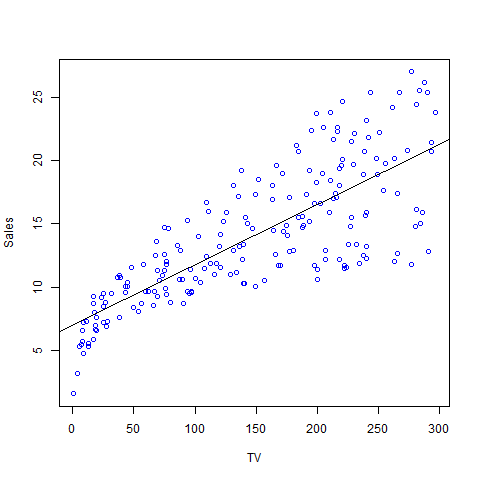
\includegraphics{images/scatterplot-tv-sales.png}
\end{figure}






\end{document}
